% Options for packages loaded elsewhere
% Options for packages loaded elsewhere
\PassOptionsToPackage{unicode}{hyperref}
\PassOptionsToPackage{hyphens}{url}
\PassOptionsToPackage{dvipsnames,svgnames,x11names}{xcolor}
%
\documentclass[
  number,
  preprint]{elsarticle}
\usepackage{xcolor}
\usepackage{amsmath,amssymb}
\setcounter{secnumdepth}{5}
\usepackage{iftex}
\ifPDFTeX
  \usepackage[T1]{fontenc}
  \usepackage[utf8]{inputenc}
  \usepackage{textcomp} % provide euro and other symbols
\else % if luatex or xetex
  \usepackage{unicode-math} % this also loads fontspec
  \defaultfontfeatures{Scale=MatchLowercase}
  \defaultfontfeatures[\rmfamily]{Ligatures=TeX,Scale=1}
\fi
\usepackage{lmodern}
\ifPDFTeX\else
  % xetex/luatex font selection
\fi
% Use upquote if available, for straight quotes in verbatim environments
\IfFileExists{upquote.sty}{\usepackage{upquote}}{}
\IfFileExists{microtype.sty}{% use microtype if available
  \usepackage[]{microtype}
  \UseMicrotypeSet[protrusion]{basicmath} % disable protrusion for tt fonts
}{}
\makeatletter
\@ifundefined{KOMAClassName}{% if non-KOMA class
  \IfFileExists{parskip.sty}{%
    \usepackage{parskip}
  }{% else
    \setlength{\parindent}{0pt}
    \setlength{\parskip}{6pt plus 2pt minus 1pt}}
}{% if KOMA class
  \KOMAoptions{parskip=half}}
\makeatother
% Make \paragraph and \subparagraph free-standing
\makeatletter
\ifx\paragraph\undefined\else
  \let\oldparagraph\paragraph
  \renewcommand{\paragraph}{
    \@ifstar
      \xxxParagraphStar
      \xxxParagraphNoStar
  }
  \newcommand{\xxxParagraphStar}[1]{\oldparagraph*{#1}\mbox{}}
  \newcommand{\xxxParagraphNoStar}[1]{\oldparagraph{#1}\mbox{}}
\fi
\ifx\subparagraph\undefined\else
  \let\oldsubparagraph\subparagraph
  \renewcommand{\subparagraph}{
    \@ifstar
      \xxxSubParagraphStar
      \xxxSubParagraphNoStar
  }
  \newcommand{\xxxSubParagraphStar}[1]{\oldsubparagraph*{#1}\mbox{}}
  \newcommand{\xxxSubParagraphNoStar}[1]{\oldsubparagraph{#1}\mbox{}}
\fi
\makeatother


\usepackage{longtable,booktabs,array}
\usepackage{calc} % for calculating minipage widths
% Correct order of tables after \paragraph or \subparagraph
\usepackage{etoolbox}
\makeatletter
\patchcmd\longtable{\par}{\if@noskipsec\mbox{}\fi\par}{}{}
\makeatother
% Allow footnotes in longtable head/foot
\IfFileExists{footnotehyper.sty}{\usepackage{footnotehyper}}{\usepackage{footnote}}
\makesavenoteenv{longtable}
\usepackage{graphicx}
\makeatletter
\newsavebox\pandoc@box
\newcommand*\pandocbounded[1]{% scales image to fit in text height/width
  \sbox\pandoc@box{#1}%
  \Gscale@div\@tempa{\textheight}{\dimexpr\ht\pandoc@box+\dp\pandoc@box\relax}%
  \Gscale@div\@tempb{\linewidth}{\wd\pandoc@box}%
  \ifdim\@tempb\p@<\@tempa\p@\let\@tempa\@tempb\fi% select the smaller of both
  \ifdim\@tempa\p@<\p@\scalebox{\@tempa}{\usebox\pandoc@box}%
  \else\usebox{\pandoc@box}%
  \fi%
}
% Set default figure placement to htbp
\def\fps@figure{htbp}
\makeatother





\setlength{\emergencystretch}{3em} % prevent overfull lines

\providecommand{\tightlist}{%
  \setlength{\itemsep}{0pt}\setlength{\parskip}{0pt}}



 
\usepackage[]{natbib}
\bibliographystyle{elsarticle-num}


\makeatletter
\@ifpackageloaded{caption}{}{\usepackage{caption}}
\AtBeginDocument{%
\ifdefined\contentsname
  \renewcommand*\contentsname{Table of contents}
\else
  \newcommand\contentsname{Table of contents}
\fi
\ifdefined\listfigurename
  \renewcommand*\listfigurename{List of Figures}
\else
  \newcommand\listfigurename{List of Figures}
\fi
\ifdefined\listtablename
  \renewcommand*\listtablename{List of Tables}
\else
  \newcommand\listtablename{List of Tables}
\fi
\ifdefined\figurename
  \renewcommand*\figurename{Figure}
\else
  \newcommand\figurename{Figure}
\fi
\ifdefined\tablename
  \renewcommand*\tablename{Table}
\else
  \newcommand\tablename{Table}
\fi
}
\@ifpackageloaded{float}{}{\usepackage{float}}
\floatstyle{ruled}
\@ifundefined{c@chapter}{\newfloat{codelisting}{h}{lop}}{\newfloat{codelisting}{h}{lop}[chapter]}
\floatname{codelisting}{Listing}
\newcommand*\listoflistings{\listof{codelisting}{List of Listings}}
\makeatother
\makeatletter
\makeatother
\makeatletter
\@ifpackageloaded{caption}{}{\usepackage{caption}}
\@ifpackageloaded{subcaption}{}{\usepackage{subcaption}}
\makeatother
\journal{Reliability Engineering & System Safety}
\usepackage{bookmark}
\IfFileExists{xurl.sty}{\usepackage{xurl}}{} % add URL line breaks if available
\urlstyle{same}
\hypersetup{
  pdftitle={A Benchmark-Integrity Audit Protocol for Conformal Battery State-of-Health Evaluation: Recent-Label Dependence, Schema-Bundle Sensitivity, and Threshold-Decision Risk},
  pdfauthor={Qingsong Shan; Qianning Liu},
  pdfkeywords={conformal prediction, uncertainty quantification, battery
state-of-health, prognostics and health management, predictive
maintenance, benchmark integrity, distribution shift},
  colorlinks=true,
  linkcolor={blue},
  filecolor={Maroon},
  citecolor={Blue},
  urlcolor={Blue},
  pdfcreator={LaTeX via pandoc}}


\setlength{\parindent}{6pt}
\begin{document}

\begin{frontmatter}
\title{A Benchmark-Integrity Audit Protocol for Conformal Battery
State-of-Health Evaluation: Recent-Label Dependence, Schema-Bundle
Sensitivity, and Threshold-Decision Risk}
\author[1]{Qingsong Shan%
%
\fnref{fn1}}
 \ead{shanqingsong@jxufe.edu.cn} 
\author[1]{Qianning Liu%
\corref{cor1}%
\fnref{fn2}}
 \ead{liuqianning@jxufe.edu.cn} 

\affiliation[1]{organization={Jiangxi University of Finance and
Economics, School of Statistics and Data Science, Key Laboratory of Data
Science in Finance and
Economics},city={Nanchang},country={China},countrysep={,},postcodesep={}}

\cortext[cor1]{Corresponding author}
\fntext[fn1]{Open Researcher and Contributor Identifier (ORCID):
0000-0001-9231-5699}
\fntext[fn2]{Open Researcher and Contributor Identifier (ORCID):
0000-0002-7654-6451}
        
\begin{abstract}
Conformal intervals for lithium-ion battery state-of-health (SOH) inform
maintenance decisions, but cross-dataset validation can conceal
measurement conditions. We develop a six-gate benchmark-integrity audit
of prediction-time information, split integrity, cell-block uncertainty,
schema controls, threshold decisions, and localization sensitivity.
Twelve analyses use 13,831 eligible records from 13,876 CALCE, NASA, and
Oxford observations. A pooled-domain, cell-held-out baseline reaches
94.8\% coverage (cell-block lower bound 94.2\%). Across six
cross-dataset tasks, method-matched removal of the most recent measured
SOH yields statistically supported coverage reductions in five tasks, by
as much as 60.4 percentage points; the remaining task and pooled-domain
baseline are compatible with no effect. The as-used schema bundle
decreases leave-NASA coverage by 12.0 percentage points and increases
false acceptance by 100.0 percentage points at the illustrative SOH
cutoff 0.90 (exact paired-cell p = 9.54e-07); an independent control
restricts interpretation to a bundle-level association. A
localized-residual comparator recovers one point-coverage failure; its
design carries no shift-robust guarantee. Each gate couples evidence
requirements to claim bounds, yielding an executable pre-submission
check demonstrated on three public battery benchmarks. Prospective
applications are needed to establish detection performance.
\end{abstract}





\begin{keyword}
    conformal prediction \sep uncertainty quantification \sep battery
state-of-health \sep prognostics and health management \sep predictive
maintenance \sep benchmark integrity \sep 
    distribution shift
\end{keyword}
\end{frontmatter}
    

\section{Introduction}\label{introduction}

Data-driven prognostics and health management (PHM) increasingly
supplies the evidence on which maintenance and serviceability decisions
rest, and closing the gap between research practice and trustworthy
deployment is a recognized priority for the reliability community
\citep{zio2022prognostics, lin2026recent}. Lithium-ion battery
state-of-health (SOH) estimation is a flagship case: high-impact
data-driven estimators are routinely evaluated on public cycle-level
datasets \citep{wang2023improved, meng2023long}, and uncertainty
quantification is now treated as a first-class evaluation criterion for
such models \citep{basora2025benchmark, nemani2023uncertainty}.
Conformal prediction --- with its finite-sample coverage guarantee ---
is entering reliability-engineering and battery pipelines
\citep{xu2026uncertaintyaware, javanmardi2023conformal, soon2026enhancing}.
Because SOH intervals feed threshold decisions about maintenance,
replacement, and second-life use, interval miscalibration has direct
decision consequences
\citep{mitici2023dynamic, zhuang2023prognostic, wang2026multiaction}.

SOH uncertainty estimates are often evaluated through cross-dataset
benchmarks, where a model calibrated on one collection is tested on
another --- a realistic proxy for the domain shift that deployed
prognostics faces \citep{nejjar2024domain}. In maintenance- and
reliability-facing uses, it is tempting to read those intervals as
evidence that threshold decisions remain trustworthy under protocol
shift. Yet dataset composition and feature choices, rather than model
quality, can drive reported battery-prognostics performance
\citep{nagulapati2021capacity, geslin2023selecting}, and the reliability
of machine-learning evidence is itself an engineering quantity that
requires pre-deployment assessment \citep{chen2024evaluating}. We
therefore treat benchmark construction and prediction-time information
as part of the reliability claim itself.

We turn this premise into an explicit, governed audit protocol and
demonstrate it on real cycle-level SOH records from the Center for
Advanced Life Cycle Engineering (CALCE), the National Aeronautics and
Space Administration (NASA), and Oxford. Within these three collections,
we ask how much of the apparent validity of conformal SOH evidence
depends on access to the most recent measured SOH, and what remains
interpretable after schema, protocol, and decision-level checks.

Two bodies of work bear directly on this question, but neither audits
the benchmark itself. Conformal methods in reliability engineering and
battery state estimation concentrate on producing or adapting predictive
intervals
\citep{xu2026uncertaintyaware, wang2025robust, javanmardi2023conformal, piao2025crulp, soon2026enhancing},
while transfer and domain-generalization methods concentrate on making
estimators survive distribution shift
\citep{nejjar2024domain, nejjar2026uncertaintyguided, fei2026decoupled}.
Non-exchangeability theory bounds how far conformal coverage can drift
\citep{barber2023beyond, oliveira2024split}, but it does not identify
which measurement-validity channel a particular benchmark contains.
Section \ref{sec-related-work} details this gap; our protocol addresses
it.

The main contributions of this paper are as follows:

\begin{enumerate}
\def\labelenumi{\arabic{enumi}.}
\tightlist
\item
  We define a benchmark-integrity audit protocol whose six governed
  gates cover the prediction-time information set, split integrity,
  cell-block uncertainty, schema negative controls, threshold-decision
  consequences, and localization sensitivity.
\item
  We quantify recent-SOH access as a load-bearing, task-dependent
  measurement condition, separating a method-selection ablation from
  method-matched, row-matched contrasts.
\item
  We audit as-used schema-bundle sensitivity with multiplicity-adjusted
  intervals and an independently permuted-feature negative control,
  showing how the control gate confines observed bundle effects to a
  sensitivity warning rather than a field-specific mechanism
  attribution.
\item
  We report a corrected leave-NASA (LNAS) schema-bundle false-acceptance
  increase of +100.0 pp (percentage points) at threshold 0.90 (exact
  paired-cell p = 9.54e-07; 21 effective cells and 1,127 records),
  linking interval behavior to threshold-decision risk under the
  bundled, noncausal interpretation.
\item
  We bound residual sensitivity with a localized-residual comparator
  envelope, distinguishing empirical recovery from a formal
  covariate-shift guarantee.
\end{enumerate}

Operationally, raw cross-dataset conformal coverage becomes battery SOH
reliability evidence only after the benchmark's prediction-time
information, split construction, uncertainty units, controls, decision
consequences, and localization have been audited. The protocol makes
that audit concrete and executable.

The remainder of the paper is organized as follows. Section
\ref{sec-related-work} reviews related work on conformal prediction,
battery SOH uncertainty, and benchmark integrity. Section
\ref{sec-methodology} defines the audit design, its provenance, and its
claim boundaries. Section \ref{sec-results} reports evidence on
recent-label dependence, schema-bundle sensitivity, residual drift,
decision consequences, and localized calibration. Section
\ref{sec-discussion} discusses implications and limitations, and Section
\ref{sec-conclusion} gives concluding remarks.

\section{Related Work}\label{sec-related-work}

\subsection{Conformal prediction: guarantees and their boundary
conditions}\label{conformal-prediction-guarantees-and-their-boundary-conditions}

Conformal prediction provides finite-sample predictive-coverage
guarantees under exchangeability
\citep{vovk2005algorithmic, lei2018distributionfree, angelopoulos2023conformal}.
Conformalized quantile regression calibrates quantile-regression
estimates to retain finite-sample coverage
\citep{romano2019conformalized}, and weighted conformal variants extend
the guarantee to covariate shift when the shift mechanism can be
estimated \citep{tibshirani2019covariate}. The boundary conditions of
these guarantees are now well mapped. When calibration and test data are
dependent or non-exchangeable, coverage deviates by an amount that
theory can bound but not eliminate
\citep{barber2023beyond, oliveira2024split}, and ensemble batch
prediction intervals extend conformal thinking to dependent time series
\citep{xu2023conformal}. Online and adaptive variants track arbitrary
distribution shifts, but they require sequential feedback after each
prediction \citep{gibbs2021adaptive, gibbs2024conformal}, which a
one-shot cross-dataset evaluation does not provide. A parallel line
sharpens the distinction between marginal and conditional validity:
exact conditional coverage is unattainable in general, and localized or
reweighted calibration offers only partial remedies
\citep{gibbs2025conformal, guan2022localized, hore2024conformal}.
Conformal risk control generalizes coverage to other monotone risks,
including decision-relevant error rates, with non-exchangeable
extensions
\citep{angelopoulos2024conformalrisk, farinhas2024nonexchangeable}.

These guarantees do not by themselves certify a reliability benchmark.
If the information set includes recent labels, dataset identity, or
bookkeeping fields unavailable in the intended decision setting, nominal
coverage can describe the constructed benchmark rather than the intended
threshold-decision problem. The localized-residual analysis used in this
paper is a diagnostic inspired by this literature, not an implementation
of density-ratio weighted conformal prediction.

\subsection{Uncertainty-aware battery SOH and remaining useful life
prognostics}\label{uncertainty-aware-battery-soh-and-remaining-useful-life-prognostics}

Battery SOH and remaining useful life (RUL) studies have long reported
probabilistic forecasts and prognostic performance under uncertainty
\citep{saxena2010evaluating, he2011remaining, liu2020futurecapacity},
and real-application SOH estimation has a mature methodological
literature \citep{berecibar2016critical}. Within the
reliability-engineering literature specifically, data-driven battery
prognostics is a flagship application: high-impact estimators define the
benchmark conventions on CALCE-, NASA-, and Oxford-style cycle datasets
\citep{wang2023improved, meng2023long, wei2023prediction}. An explicitly
uncertainty-aware thread now reports quantile intervals validated on the
same public datasets \citep{zhang2024reliability}, Bayesian-calibrated
SOH uncertainty under deployment shift \citep{zhu2025bayesian},
probabilistic degradation-trajectory health assessment
\citep{che2024predictive, lin2023battery}, and recent dynamical-model
variants \citep{wang2025remaining}. Label scarcity at deployment is a
recognized constraint in this literature: adaptive prediction with few
or no in-service capacity labels is studied as its own problem
\citep{zhang2022adaptive, pan2024probabilistic}, which makes the
availability of a recent measured SOH a substantive modeling assumption
rather than a technicality. Dedicated benchmarks and reviews now treat
uncertainty quantification as a first-class evaluation criterion for
deep-learning prognostics
\citep{basora2025benchmark, lin2026recent, nemani2023uncertainty, salinascamus2025comprehensive}.

Conformal prediction itself has entered this application class in three
roles. It produces calibrated RUL and degradation intervals
\citep{xu2026uncertaintyaware, liu2026credible, javanmardi2023conformal, piao2025crulp, soon2026enhancing},
adapts interval inference to corrupted inputs or engineering-design
uncertainty \citep{wang2025robust, wu2026sequential}, and supports
anomaly detection or width-aware calibration
\citep{yuan2026conformal, xu2026widthoptimized}. Related industrial
time-series work also documents the exchangeability violations that
motivate such adaptations \citep{zhang2025uncertainty}. These methods
improve or diagnose interval estimators while largely taking benchmark
construction as fixed; our audit puts that construction to the test.

\subsection{Cross-dataset evaluation, transfer, and domain shift in
prognostics and health
management}\label{cross-dataset-evaluation-transfer-and-domain-shift-in-prognostics-and-health-management}

Transfer research pursues several remedies for distribution shift.
Domain-adaptation methods move SOH or RUL estimators across batteries,
operating profiles, and laboratory or field domains
\citep{ye2021domainadversarial, vilsen2022field, shen2024review, nejjar2024domain, nejjar2026uncertaintyguided, wang2026twostage}.
Condition-aware and domain-generalization methods target fleet or
protocol variation \citep{zhang2023multitask, fei2026decoupled}, while
adjacent reliability work mitigates shift in data-driven risk assessment
\citep{wang2025mitigating}. These studies focus on remedies and
generally treat the benchmark schema as a fixed prerequisite for
comparison. We take the complementary audit-side view: before asking
whether a model transfers, we ask whether the benchmark's information
set, splits, feature schema, and decision endpoints support the
reliability conclusion being drawn.

\subsection{Benchmark integrity, leakage, and evaluation
validity}\label{benchmark-integrity-leakage-and-evaluation-validity}

Machine-learning reliability research warns that apparent predictive
performance can be driven by unintended signals, undocumented data
provenance, or data-splitting and feature-availability choices
\citep{gebru2021datasheets, geirhos2020shortcut, kapoor2023leakage}. The
battery and PHM literatures now contain concrete instances: feature
selection can produce misleading battery-lifetime predictions
\citep{geslin2023selecting}, training-set size and composition ---
rather than model class --- can drive reported capacity-estimation
accuracy \citep{nagulapati2021capacity}. Explainability analysis reveals
which features an SOH model actually exploits
\citep{wang2023explainabilitydriven}, and open benchmark suites codify
the feature schemas whose integrity this paper audits
\citep{wang2024open}. Within reliability engineering, an
evaluation-validity genre is emerging: simple baselines can expose what
domain-shift benchmarks actually measure in condition monitoring
\citep{panic2027simple}, and pre-deployment reliability assessment of
machine-learning evidence is treated as its own engineering problem
\citep{chen2024evaluating}.

We found no integrated audit protocol in the literature reviewed above
that treats a conformal SOH benchmark itself as the object of
reliability analysis. We therefore analyze the benchmark evidence
directly: how conformal interval behavior and threshold decisions change
across recent-label, split, schema-bundle, residual-drift, and
SOH-threshold diagnostics. Six gates organize these diagnostics, each
with an explicit evidentiary requirement and a corresponding bound on
the admissible claim.

\section{Methodology}\label{sec-methodology}

We develop a governed benchmark-integrity audit protocol for conformal
SOH evidence. Table \ref{tbl-audit-protocol} defines six gates, each
linking a measurement condition to the evidence it requires and the
consequence of failure. The protocol grew from a sequence of completed
diagnostic analyses. Component decision rules were recorded in the
corresponding experiment plans before execution; the six-gate synthesis
was developed afterward and is therefore not prospectively registered. A
failed gate narrows the resulting claim without discarding a negative or
heterogeneous result. The remainder of this section defines the
protocol's gates, decision rules, and interpretation boundaries.

\begin{table}

\caption{\label{tbl-audit-protocol}Governed benchmark-integrity audit protocol for conformal SOH evidence. Each gate names the measurement condition examined, the evidence required, and the consequence of failure applied in this audit.}

\centering{

\centering
\scriptsize


\begin{tabular}{>{\raggedright\arraybackslash}p{0.22\linewidth}>{\raggedright\arraybackslash}p{0.46\linewidth}>{\raggedright\arraybackslash}p{0.24\linewidth}}
\toprule
Gate & Evidence required & Consequence of failure \\
\midrule
G1 Information set & State whether recent measured SOH or another oracle label is available at prediction time & No claim for settings without recent labels \\
G2 Split integrity & Verify task-appropriate disjoint training, validation, calibration, and test indices; require cell-disjoint histories where the task claims cell-level holdout & Treat coverage as split-contingent \\
G3 Uncertainty units & Report cell-block uncertainty rather than row-level i.i.d. intervals & Treat uncertainty as optimistic \\
G4 Schema sensitivity & Compare schema contrasts with an independent permuted-feature control and multiplicity adjustment & Bundle-level warning; no mechanism claim \\
G5 Decision consequences & Report threshold false acceptance and false rejection with record denominators, effective cell counts, and sparse-cell flags & Do not promote coverage to serviceability evidence \\
G6 Localization sensitivity & Compare standard and localized calibration as a sensitivity envelope & Failure: no empirical recovery; apparent success: point-coverage sensitivity only. Neither outcome authorizes a shift-robust claim without a guarantee-bearing method and verified assumptions \\
\bottomrule
\end{tabular}

}

\end{table}%

We organize the evidence around governed diagnostic analyses and
generate every reported value from a scripted results table. All active
rows are real battery state-of-health records from CALCE, NASA, and
Oxford
\citep{calce_battery_data, nasa_pcoe_battery_data, howey2017oxford}; the
analysis contains no synthetic records. The methodological contribution
is the protocol used to audit the benchmark evidence constructed from
these public cycle-level datasets. The 12 completed diagnostic analyses
comprise a pooled-domain, cell-held-out coverage baseline, a
recent-label ablation, a cross-protocol transfer diagnostic, a
residual-bias screen, which tests whether calibration residual signs
vary systematically with cycle position, a host-timing screen, which
tests whether results shift with the wall-clock execution host, and a
negative-control check. The remaining analyses comprise a method-family
comparison, a threshold decision-utility audit, a schema-cleaning audit,
a hard-regime audit, a schema-to-decision audit, and a
localized-residual comparator. Supplementary Tables S1--S2 map every
analysis to its gate, task, feature schema, method family, parameter
grid, selection rule, seed, plan identifier, governed rerun, and
deviation record. The archived plans and regeneration sources are
preserved in the public replication repository.

The physical case spans three laboratory platforms rather than one
nominally homogeneous fleet. The CALCE subset contains six CS2 (1.10 Ah)
and six CX2 (1.35 Ah) small prismatic cells with LiCoO\(_2\) cathodes.
The archive documents constant-current/constant-voltage charging for CS2
and 0.5 C or 1 C constant-current discharge for the selected CS2/CX2
cells; the retained row files do not encode ambient temperature
\citep{calce_battery_data}. The NASA subset contains 25 Li-ion cells
from multiple Prognostics Center of Excellence batches; the repository
describes charge, discharge, and impedance profiles for nominal 2-Ah
cells, and the retained metadata cover chamber temperatures of 4, 22,
24, and 43 \(^\circ\)C, but do not consistently encode cathode chemistry
\citep{nasa_pcoe_battery_data}. Oxford contributes eight 740-mAh Kokam
pouch cells aged in a 40 \(^\circ\)C chamber with
constant-current/constant-voltage charging and an ARTEMIS urban-drive
discharge profile \citep{howey2017oxford}. These differences make label
and protocol comparability part of the audit boundary rather than a
solved preprocessing detail. Table \ref{tbl-datasets} summarizes the
45-cell source evidence base of 13,876 cycle rows and the 13,831 rows
eligible for a strictly prior recent-SOH feature.

\begin{table}

\caption{\label{tbl-datasets}Real battery datasets after preprocessing. Rows are source/eligible; every eligible row has an earlier same-cell SOH record.}

\centering{

\centering
\scriptsize


\begin{tabular}{l>{\raggedright\arraybackslash}p{0.27\linewidth}>{\raggedright\arraybackslash}p{0.31\linewidth}rcc}
\toprule
Dataset & Cell platform & Cycling / temperature & Cells & Rows & SOH range \\
\midrule
CALCE & CS2/CX2 prismatic, LiCoO$_2$, 1.10/1.35 Ah & CS2: CC--CV charge; selected CS2/CX2: 0.5C/1C discharge; temperature absent & 12 & 11{,}604/11,592 & 0.40--1.01 \\
NASA & Multi-batch Li-ion cells; archive nominal 2 Ah; cathode not consistently encoded & Charge/discharge/EIS; retained metadata span 4--43 $^\circ$C & 25 & 1{,}753/1,728 & 0.41--1.00 \\
Oxford & Kokam SLPB533459H4 pouch, 0.74 Ah & CC--CV charge; ARTEMIS urban-drive discharge; chamber 40 $^\circ$C & 8 & 519/511 & 0.62--1.00 \\
\midrule
Total & Three public laboratory platforms & Heterogeneous protocols and measurement conventions & 45 & 13,876/13,831 & 0.40--1.01 \\
\bottomrule
\end{tabular}

}

\end{table}%

The seven evaluation tasks use the same model families but change the
target-domain role. Task abbreviations use Main for the pooled-domain,
cell-held-out task, and leave-CALCE (LCAL), target-recalibrated CALCE
(TCAL), leave-NASA (LNAS), target-recalibrated NASA (TNAS), leave-Oxford
(LOxf), and target-recalibrated Oxford (TOxf) for the six cross-dataset
tasks. Leave-domain-out tasks fit, select, and calibrate on the other
two domains and test on all eligible rows of the named held-out domain.
Target-recalibrated tasks add early target-domain rows: progress 0--20\%
enters training, 20--35\% calibration, 35--55\% validation, and rows
after 55\% form the test set. These boundaries are pairwise disjoint.
Table \ref{tbl-task-design} reports the resulting row counts; the
held-out target contains 12 CALCE, 25 NASA, or 8 Oxford cells, while
Main uses 10 test cells. Main is a pooled-domain within-benchmark
baseline: all three datasets contribute to fitting and test sets, while
cell identities remain disjoint; it is not a single-physical-protocol
validation.

\begin{table}

\caption{\label{tbl-task-design}Operational task construction and row counts for training, calibration, validation, and testing.}

\centering{

\centering
\scriptsize


\begin{tabular}{llrl}
\toprule
Task & Construction & Test cells & Train/Cal/Val/Test rows \\
\midrule
Main & Cell-disjoint mixed-domain held-out split & 10 & 7961/880/680/2323 \\
LCAL & Other domains to all CALCE rows & 12 & 1122/241/116/11592 \\
TCAL & Other domains + early CALCE to late CALCE & 12 & 4566/1754/2344/5167 \\
LNAS & Other domains to all NASA rows & 25 & 7082/664/636/1728 \\
TNAS & Other domains + early NASA to late NASA & 25 & 12447/279/322/783 \\
LOxf & Other domains to all Oxford rows & 8 & 7718/855/608/511 \\
TOxf & Other domains + early Oxford to late Oxford & 8 & 13421/71/106/233 \\
\bottomrule
\end{tabular}

}

\end{table}%

The Main row counts follow governed cell partitions and the progress
windows specified below. Leave-domain-out tasks reuse those partitions
after restricting training, calibration, and validation to non-target
domains; consequently, their source-domain rows need not account for
every eligible source-domain row in Table \ref{tbl-datasets}.
Target-recalibrated boundaries are time-forward and pairwise
row-disjoint.

Main is a seed-42, domain-stratified cell split, not a within-cell
forecasting split. Within each domain, shuffled cells are assigned
55\%/20\%/10\%/remainder to training/calibration/validation/test;
calibration retains progress at most 0.55 and test retains progress at
least 0.35. The four cell sets are disjoint, and no test cell
contributes an earlier row to model fitting, selection, or calibration.
The complete cell membership is recorded below; the governed split
manifest preserves row indices together with the manifest checksum.

\begin{quote}
\scriptsize
\textbf{Complete Main split membership} (domain entries are row counts).\par
\textbf{Train} (7,961 rows; CALCE 6,839; NASA 879; Oxford 243): CALCE\_CS2\_33, CALCE\_CS2\_36, CALCE\_CX2\_33, CALCE\_CX2\_34, CALCE\_CX2\_36, CALCE\_CX2\_38, NASA\_B0007, NASA\_B0025, NASA\_B0026, NASA\_B0028, NASA\_B0029, NASA\_B0031, NASA\_B0042, NASA\_B0043, NASA\_B0048, NASA\_B0053, NASA\_B0054, NASA\_B0055, NASA\_B0056, Oxford\_Cell1, Oxford\_Cell3, Oxford\_Cell4, Oxford\_Cell6.

\textbf{Cal} (880 rows; CALCE 639; NASA 216; Oxford 25): CALCE\_CS2\_35, CALCE\_CS2\_38, NASA\_B0006, NASA\_B0027, NASA\_B0045, NASA\_B0046, NASA\_B0047, Oxford\_Cell5.

\textbf{Val} (680 rows; CALCE 564; NASA 44; Oxford 72): CALCE\_CS2\_37, NASA\_B0032, NASA\_B0051, Oxford\_Cell2.

\textbf{Test} (2,323 rows; CALCE 1,968; NASA 255; Oxford 100): CALCE\_CS2\_34, CALCE\_CX2\_35, CALCE\_CX2\_37, NASA\_B0005, NASA\_B0018, NASA\_B0030, NASA\_B0044, NASA\_B0049, Oxford\_Cell7, Oxford\_Cell8.
\end{quote}

For cell \(i\) and recorded cycle \(t\), \texttt{prev\_soh} is
\(SOH_{i,t-1}\): the immediately preceding recorded same-cell
capacity-SOH after sorting by dataset, cell identifier, and cycle index.
The \(t-1\) measurement must occur before the prediction event at \(t\).
Each cell's first row has no such measurement and is excluded before
every split is constructed (45 rows in total); no same-row target fill
or other imputation is used. Thus, the recent measured SOH is an oracle
only in the sense that it assumes a previous capacity measurement is
actually available at prediction time, not because it accesses
\(SOH_{i,t}\).

The primary nominal coverage level is 90\%. This paper reports coverage,
width, dependence-aware uncertainty, threshold decision utilities,
schema diagnostics, and localized-residual comparator outcomes from the
scripted results table. Before the schema-to-decision analysis was
executed, its experiment plan defined five contrasts across seven tasks
and seven endpoints: one coverage endpoint plus the predeclared SOH
thresholds 0.65, 0.70, 0.75, 0.80, 0.85, 0.90, giving 245 tests.
Coverage and false-acceptance deltas in Tables \ref{tbl-schema-deltas}
and \ref{tbl-false-acceptance-deltas} use Bonferroni-adjusted, SE-based
normal intervals from 1000 cell-block resamples; the family-wise level
0.05 gives a per-test level near \(2\times10^{-4}\) and \(z \approx\)
3.7. Zero-SE boundaries use the exact paired-cell sign test. By
contrast, the Main 94.2\%--97.1\% interval and the lower bounds in Table
\ref{tbl-adaptive-envelope} are 2.5/97.5-percentile cell-block bootstrap
intervals, while Table \ref{tbl-decision-tradeoff} reports uncorrected
95\% cell-block normal intervals. The limited number of battery-cell
blocks makes extreme-tail normal widths uncertain; this is an additional
reason to treat coverage flags as sensitivity signals and require a
negative-control gate. The same data interface generates text, tables,
and captions to avoid manual transcription.

The nominal target is the evaluation criterion, while each conformal
variant selects its calibration quantile strictly on a disjoint
validation split and never tunes on the test set. For the pooled-domain,
cell-held-out diagnostic baseline, the selected operating point uses
\(q\)-level 0.93 and realizes test coverage of 94.8\%. We use this
over-coverage as the baseline's `apparent reliability' before domain
shift or artifact removal and as the reference for subsequent
measurement-validity checks against the 90\% target.

We use persistence-anchor behavior as a diagnostic probe of recent-label
and anchor dependence. Cross-protocol failures then become validity
evidence: a failure that persists after schema cleaning is consistent
with residual protocol drift, whereas a small, directionally
heterogeneous, or control-inconsistent schema effect limits the schema
inference. Recent-label dependence and residual drift cannot be fully
separated in this evidence base, so residual drift remains an explicit
boundary of interpretation.

The audit examines four diagnostic dimensions:

\begin{enumerate}
\def\labelenumi{\arabic{enumi}.}
\tightlist
\item
  recent-label / anchor dependence;
\item
  as-used schema-bundle sensitivity;
\item
  residual protocol drift after schema checks;
\item
  SOH serviceability-threshold decision risk under finite-cell evidence.
\end{enumerate}

The Main pooled-domain, cell-held-out diagnostic baseline is the
selected persistence-anchor Mondrian conformal predictor
\citep{vovk2005algorithmic}; the split-conformal constructions and
coverage definitions follow standard practice
\citep{angelopoulos2023conformal}. The diagnostic families include
quantile regression (QR), conformalized quantile regression (CQR)
\citep{romano2019conformalized}, and natural-gradient boosting (NGBoost)
\citep{duan2020ngboost}. For the no-recent-SOH condition, validation
selects a gradient-boosting domain-Mondrian conformal variant, a
group-conditional calibration construction suited to settings where
exchangeability across domains is not credible \citep{barber2023beyond}.
We use this condition to measure the benchmark's dependence on
recent-label access.

The calibration-selection rule chooses the operating point within each
condition, so the full-feature and no-recent-SOH conditions can select
different conformal families. Their pooled-domain coverage difference
measures the complete selection pipeline's response to removing recent
labels, whereas the row-matched comparison in Section \ref{sec-results}
supplies the same-method feature-isolation contrast. We use
gradient-boosting CQR for decision-utility diagnostics, schema
comparisons, and the localized-residual comparator. Training,
validation, calibration, and test indices are pairwise disjoint within
each task.

The as-used bundle contains \texttt{source\_row\_id},
\texttt{target\_cycle\_index}, and the permuted control column, whereas
the clean-original schema removes all three. The bundle contrast
therefore identifies their joint effect rather than a
bookkeeping-specific mechanism. The independent control adds a
fixed-seed (seed 1033) permutation of \texttt{log\_cycle\_index} to the
clean schema and refits the complete pipeline on the same rows. Because
this control uses one permutation draw (\(B=1\)) rather than a sampled
permutation null distribution, it serves only as a veto on mechanism
attribution.

A decision-risk cell is defined relative to a capacity-SOH
serviceability threshold and a predicted SOH interval with lower bound
\(L\) and upper bound \(U\) for a test record with true SOH \(y\). The
record is threshold-acceptable when its lower bound \(L\) is at or above
the threshold, threshold-unacceptable when its upper bound \(U\) is
below the threshold, and uncertain when the interval straddles the
threshold. A false-acceptance event is a threshold-acceptable record
whose true SOH \(y\) is below the threshold; a false-rejection event is
a threshold-unacceptable record whose true SOH \(y\) is at or above the
threshold. The reported false-acceptance rate divides false-acceptance
events by the number of actually threshold-unacceptable records, the
false-rejection rate divides false-rejection events by the number of
actually threshold-acceptable records, and the uncertain rate divides
uncertain records by all records. Each rate carries a cell-block
bootstrap confidence interval that resamples battery cells with
replacement. When every contributing cell block contains zero events,
that bootstrap has zero empirical variance; the table therefore marks
the interval as bootstrap-degenerate rather than displaying a zero-width
confidence interval. Such a boundary is not evidence of zero underlying
risk. Auditing these monotone decision risks alongside coverage follows
the same motivation as conformal risk control, which generalizes
coverage guarantees to decision-relevant error rates
\citep{angelopoulos2024conformalrisk}. These thresholds are
capacity-based decision cutoffs, not demonstrated electrochemical or
thermal safety boundaries. To avoid over-reading sparse cells, a
small-denominator suppression rule flags any decision cell whose
denominator is below 5 as exploratory rather than as a headline rate.

Schema-bundle sensitivity is adjudicated by a rule documented before the
schema-to-decision analysis and applied identically to every task. A
task is flagged when the as-used-minus-clean coverage interval excludes
zero and the absolute delta is at least 3 pp (percentage points). This
flag is necessary but not sufficient for a mechanistic claim: the
independent permuted-feature control must remain null across both its
coverage contrast and all six false-acceptance endpoints. The bundle's
false-acceptance-rate delta is evaluated separately with multiplicity
adjustment or, for zero-standard-error boundaries, an exact paired-cell
sign test; cells below 5 effective observations are exploratory. This
hierarchy prevents a bundled association from being relabeled as a
bookkeeping mechanism, while still allowing a corrected bundle-level
decision association to be reported without field-specific attribution.

Two dependence boundaries govern interpretation. First, the conformal
calibration objects are cycle-level residuals from longitudinal cell
records, so exchangeability depends on the task construction and does
not extend automatically to independent operating histories. Under such
dependence, theory bounds but does not eliminate deviations from nominal
split-conformal coverage \citep{oliveira2024split, xu2023conformal}. We
therefore resample cells as blocks and interpret the resulting intervals
as dependence-aware diagnostics; a fully cell-independent prospective
forecasting design would provide stronger evidence. Second, the main
dependence probe treats recent-SOH as an oracle recent label. It is a
legitimate autoregressive measurement in a laboratory setting where
previous capacity has just been measured, but it may be unavailable to
an online battery-management system. We therefore treat recent-SOH
access as a measurement condition that must be declared, rather than
labeling it as leakage in every setting.

The SOH label is capacity-normalized within the harmonized project data
interface, following the conventions of published SOH benchmark suites
on these datasets \citep{wang2024open, zhang2024reliability}, and Table
\ref{tbl-datasets} reports the ranges after quality assurance. Because
the source datasets differ in cycling protocol, temperature range, and
capacity measurement practice, label comparability forms part of the
benchmark-validity boundary. We do not vary denominators, smoothing
rules, or anomaly-removal policies here; attributing every cross-dataset
coverage failure to physical protocol drift or model behavior would
require that additional sensitivity analysis to be run.

To test whether a standard conformal failure is sensitive to residual
localization, we also evaluate a heuristic localized-residual CQR
comparator in the spirit of localized conformal prediction
\citep{guan2022localized}. Calibration and target features are
standardized by calibration means and standard deviations. For target
row \(x\), calibration score \(r_i\) receives Gaussian weight
\(w_i(x)=\exp\{-d_i(x)^2/(2h^2)\}+10^{-12}\), where \(d_i^2\) is the
mean squared standardized distance over the recorded common shift
features. The local radius is the weighted conformal quantile. Bandwidth
\(h\in\{0.25,0.50,1,2,4,\infty\}\) is selected only on validation data
by the predeclared coverage-first-then-width objective; test metrics are
not used. The comparator is motivated by covariate-shift conformal work
\citep{tibshirani2019covariate}, but it neither estimates a density
ratio nor carries a formal covariate-shift guarantee. Meeting the
envelope means that point coverage reaches nominal; a lower-bound
shortfall is recorded only when the standard percentile lower bound is
below nominal and the localized lower bound is at or above it. We use
the result as a sensitivity diagnostic, not as a method comparison.

\section{Results}\label{sec-results}

We apply the audit protocol to a cross-dataset conformal SOH benchmark
and examine the reliability evidence it produces. The analysis tracks
how interval coverage and SOH threshold decisions change with
recent-label access, split construction, feature-schema sensitivity,
residual protocol drift, and localized residual weighting.

The evidence base is a set of diagnostic contrasts over the same
real-data benchmark splits. Task abbreviations follow Section
\ref{sec-methodology}: Main denotes the pooled-domain, cell-held-out
task. Table \ref{tbl-evidence-map} reports the argument-bearing
contrasts needed to interpret reliability evidence; ancillary timing and
residual-stress screens are treated as robustness checks rather than
headline findings.

\begin{table}

\caption{\label{tbl-evidence-map}Gate-by-gate audit ledger. Later tables report interval estimates. Pass* denotes complete reporting with bounded interpretation; pp denotes percentage points.}

\centering{

\centering
\scriptsize


\begin{tabular}{>{\raggedright\arraybackslash}p{0.05\linewidth}>{\raggedright\arraybackslash}p{0.50\linewidth}>{\raggedright\arraybackslash}p{0.10\linewidth}>{\raggedright\arraybackslash}p{0.25\linewidth}}
\toprule
Gate & Case evidence & Verdict & Claim bound \\
\midrule
G1 & Prior SOH declared; removal -60.4 pp in TCAL; TOxf +4.3 pp with interval including zero & Conditional & Exclude settings without prior labels \\
G2 & Main cell-disjoint, governed source splits for leave-domain tasks, forward disjoint recalibration rows & Pass & Split-contingent \\
G3 & Cell-block intervals, effective cell counts 8--25 across tasks & Pass & No row-i.i.d. precision \\
G4 & LCAL/LNAS bundle effects, LNAS -12.0 pp, control non-null in LCAL/TCAL & Fail & Bundle only, no mechanism \\
G5 & Both threshold errors, uncertainty status, cell/record counts, no sparse displayed cell & Pass* & Illustrative, not deployment rates \\
G6 & TNAS recovers one point failure, Main/LCAL decrease, no lower-bound shortfall recovered & Bounded diagnostic & One point failure recovered; no lower-bound recovery or formal guarantee \\
\bottomrule
\end{tabular}

}

\end{table}%

The selected Main baseline is the persistence-anchor Mondrian conformal
diagnostic. On the pooled-domain, cell-held-out task it reaches coverage
94.8\% with CI 94.2\%-97.1\%, mean width 0.038, and sample size 2,323.
The ablation package performs a separate validation-only selection: its
full-feature reference selects the persistence-anchor standard conformal
diagnostic, with coverage 92.6\% and mean width 0.027. Removing the
recent-SOH feature changes that within-package selection to the
gradient-boosting domain-Mondrian conformal diagnostic, with coverage
80.8\% and mean width 0.221; relative to the stated ablation reference,
the coverage change is -11.8 pp and the width increase is 0.193.
Accordingly, these deltas use the ablation reference rather than the
separately selected Main baseline. Figure \ref{fig-evidence-flow}
summarizes the audit logic: raw coverage is interpreted only after its
measurement conditions are examined.

\begin{figure}[!htbp]
\centering
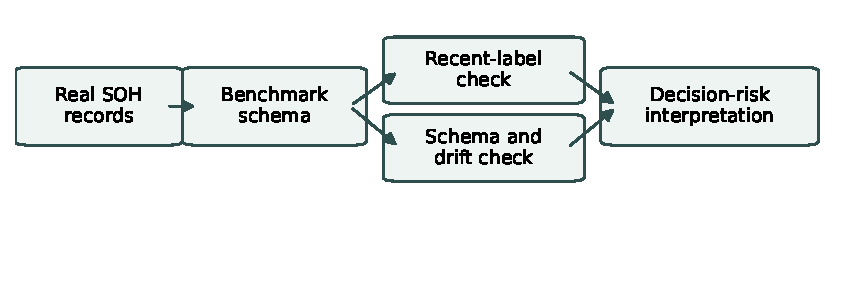
\includegraphics[width=0.95\linewidth]{figures/evidence-flow.pdf}
\caption{The six-gate benchmark-integrity audit converts an unmet evidence requirement into a narrower admissible claim rather than a stopped analysis. Case verdicts are shown inside the gates; dashed orange or vermilion borders mark conditional, bounded-diagnostic, or failed gates. Pass* means that G5's reporting requirements are met while its serviceability interpretation remains bounded.}
\label{fig-evidence-flow}
\end{figure}

The cross-protocol results vary across uncertainty families and interval
widths. Same-split QR/CQR/NGBoost comparisons show that higher coverage
can require a different uncertainty family or wider intervals; for
example, in the main held-out task, CQR is coverage-aligned but has 2.72
times the persistence-anchor width. In the common-cycle, no-recent-label
audit, coverage is 92.9\% on Main, 29.5\% on LNAS, and 3.1\% on LOxf.
This heterogeneity rules out a universal monotone benefit of recent
labels. On Main, the clean-original no-recent schema attains coverage of
92.4\%. Because the as-used no-recent schema is flagged as contaminated
in two tasks, we base the conclusions on row-matched common-schema
contrasts rather than the contaminated hard-regime rows. We retain the
host-timing and residual-bias screens as robustness checks and draw no
hardware or physical-degradation inference from them.

The method-matched recent-label delta is gradient-boosting CQR coverage
under the common no-recent-SOH schema minus coverage with the recent-SOH
reference, evaluated on identical task rows. This comparison is
heterogeneous across tasks, which is central to the measurement-validity
interpretation. Table \ref{tbl-schema-deltas} reports it beside the
as-used schema-bundle contrast and its independent permuted-feature
control.

\begin{table}

\caption{\label{tbl-schema-deltas}Task-wise coverage sensitivity (pp; Bonferroni-adjusted cell-block normal intervals). Cells/rows gives effective cells and test records. Recent is no-recent minus recent-SOH; Bundle is as-used minus clean; Control is the permuted-feature contrast. G4 fails for any non-null control endpoint.}

\centering{

\centering
\scriptsize


\begin{tabular}{lllllcc}
\toprule
Task & Cells/rows & No-recent $-$ recent & Bundle & Control & Flag & G4 control \\
\midrule
Main & 10/2,323 & +1.3 [-18.7, +21.4] & -4.1 [-21.6, +13.4] & -1.1 [-3.0, +0.7] & No & Pass \\
LCAL & 12/11,592 & -10.1 [-16.8, -3.3] & +3.2 [+1.2, +5.1] & -0.6 [-1.0, -0.2] & Yes & Fail \\
TCAL & 12/5,167 & -60.4 [-73.6, -47.2] & -2.2 [-6.9, +2.6] & -0.0 [-2.7, +2.6] & No & Fail \\
LNAS & 25/1,728 & -31.9 [-40.7, -23.1] & -12.0 [-20.5, -3.4] & -1.0 [-2.0, +0.1] & Yes & Pass \\
TNAS & 25/783 & -41.5 [-73.4, -9.7] & -10.0 [-31.2, +11.2] & -0.1 [-1.6, +1.3] & No & Pass \\
LOxf & 8/511 & -37.6 [-53.1, -22.0] & +0.4 [-0.5, +1.3] & -0.2 [-1.0, +0.6] & No & Pass \\
TOxf & 8/233 & +4.3 [-1.6, +10.2] & +0.0 [+0.0, +0.0] & -0.4 [-2.1, +1.2] & No & Pass \\
\bottomrule
\end{tabular}

}

\end{table}%

The Control column in Table \ref{tbl-schema-deltas} displays the
coverage endpoint. TCAL's G4 control failure instead occurs at the
illustrative SOH cutoff 0.85, where the clean-original minus fixed-seed
permuted-control false-acceptance contrast is -26.4 pp {[}-52.1, -0.8{]}
after Bonferroni adjustment. The largest method-matched recent-label
contrast occurs in TCAL, where removing the recent-SOH reference changes
coverage by 60.4 pp; LNAS changes by 31.9 pp.~Across the six
cross-dataset tasks, five adjusted intervals support coverage
reductions; the TOxf estimate is positive but its interval includes
zero, as does Main's. The evidence therefore establishes task-dependent
magnitudes, not a supported positive reversal. Because these comparisons
hold the conformal family and task rows fixed, they isolate
information-set sensitivity more cleanly than the selection-changing
Main ablation described above. The Main ablation changes coverage by
-11.8 pp, but its selection rule switches conformal families and
therefore measures the response of the complete selection pipeline, not
a same-method feature effect.

The as-used schema-bundle contrast passes the experiment-level coverage
flag in 2 tasks: LCAL, LNAS. LNAS coverage changes by -12.0 pp; its
maximum standardized mean difference falls from 7.15 in the raw schema
to 1.32 in the common schema. The as-used bundle, however, jointly
changes \texttt{source\_row\_id}, \texttt{target\_cycle\_index}, and the
permuted control column, and the independent permuted-feature control is
non-null in LCAL, TCAL. G4 therefore identifies bundle sensitivity but
cannot assign it to a bookkeeping field: schema identity, finite-cell
structure, and residual shift remain entangled. The failed control
vetoes the stronger artifact-mechanism interpretation.

LNAS shows a multiplicity-adjusted schema-bundle false-acceptance
increase of +100.0 pp at SOH threshold 0.90: the rate is 100.0\% under
the as-used schema and 0.0\% under the clean schema over 1,127 actually
threshold-unacceptable records and 21 effective cells (exact paired-cell
p = 9.54e-07). The bundle's decision effect is directionally
heterogeneous. The largest LCAL contrast is -100.0 pp at SOH 0.65 (0.0\%
as-used versus 100.0\% clean; 1,936 records, 12 effective cells and 12
discordant cells; exact paired-cell p = 4.88e-04), which is
risk-decreasing and does not survive multiplicity correction. Only LNAS
passes correction, and the opposite LCAL direction shows that the bundle
is not uniformly risk-increasing. Table
\ref{tbl-false-acceptance-deltas} reports the largest observed eligible
contrast for each task, and the complete 245-contrast ledger remains in
the machine-readable results archive. We therefore report bundle-level
decision associations rather than bookkeeping-specific effects or
deployment-safety rates. Table \ref{tbl-decision-tradeoff} supplies the
corresponding absolute decision risks, and Figure
\ref{fig-coverage-deltas} visualizes the task-dependent information-set
and schema-bundle sensitivities.

\begin{table}

\caption{\label{tbl-false-acceptance-deltas}Largest eligible schema-bundle false-acceptance contrast by task (pp). As-used/clean gives the two base rates (percent); cells/rows gives the effective cell blocks and actually threshold-unacceptable records; discordant is the number of nonzero paired-cell differences. Intervals are Bonferroni-adjusted and are omitted where the cell-level standard error is zero; those cells instead show exact paired-cell p-values. Only LNAS passes correction.}

\centering{

\centering
\scriptsize


\begin{tabular}{llllllll}
\toprule
Task & Delta [CI] & As-used/clean & SOH & Cells/rows & Discordant & Exact p & Corrected? \\
\midrule
Main & +4.4 [-35.9, +44.6] & 6.0/1.7 & 0.75 & 7/712 & 4 & -- & No \\
LCAL & -100.0 & 0.0/100.0 & 0.65 & 12/1,936 & 12 & 4.88e-04 & No \\
TCAL & +21.5 [-25.9, +68.8] & 28.6/7.1 & 0.85 & 12/5,036 & 9 & -- & No \\
LNAS & +100.0 & 100.0/0.0 & 0.90 & 21/1,127 & 21 & 9.54e-07 & Yes \\
TNAS & +45.8 [-19.8, +100.0] & 97.6/51.7 & 0.75 & 14/288 & 8 & -- & No \\
LOxf & +0.0 & 0.0/0.0 & 0.90 & 8/342 & 0 & 1.000 & No \\
TOxf & +0.0 & 0.0/0.0 & 0.90 & 8/233 & 0 & 1.000 & No \\
\bottomrule
\end{tabular}

}

\end{table}%

\begin{figure}[!htbp]
\centering
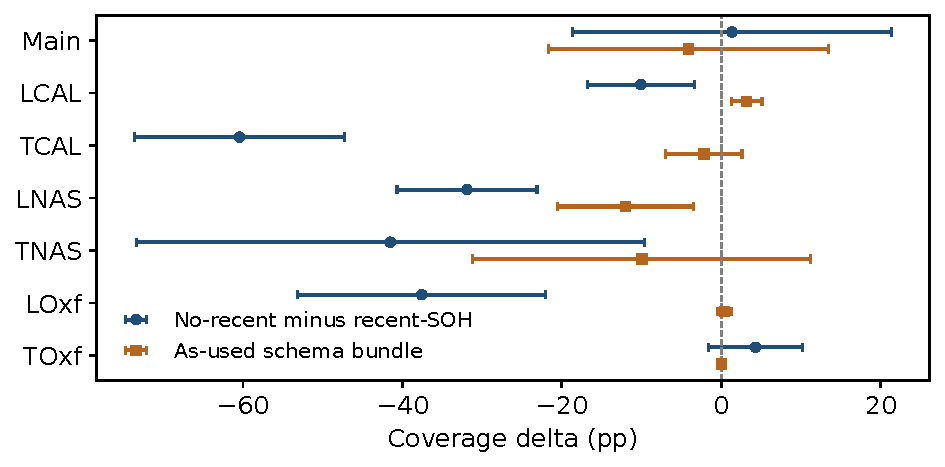
\includegraphics[width=0.9\linewidth]{figures/coverage-deltas.pdf}
\caption{Per-task recent-label and as-used schema-bundle coverage deltas (percentage points) with Bonferroni-corrected normal intervals. Recent-label deltas are large and negative in several tasks; bundle deltas are smaller, with LCAL and LNAS meeting the coverage flag. The endpoint-wide negative-control gate fails in LCAL and TCAL. The dashed line marks zero.}
\label{fig-coverage-deltas}
\end{figure}

We report decision-utility rates with their denominators and cell-block
intervals. False-acceptance and false-rejection events follow the
Section \ref{sec-methodology} definitions. Table
\ref{tbl-decision-tradeoff} reports representative decision cells at SOH
threshold 0.80. It shows why coverage alone is insufficient: the
leave-NASA CQR cell has a lower false-acceptance point estimate but
leaves a large uncertain region, whereas NGBoost exhibits a high
false-acceptance rate. These cells provide boundary evidence for the
audit; operational use requires threshold-specific validation.

\begin{table}

\caption{\label{tbl-decision-tradeoff}Illustrative threshold-0.80 decision cells (percent; uncorrected 95\% cell-block CI). c/n gives effective cells/records; BD marks a bootstrap-degenerate all-zero boundary, and Sparse denotes any denominator below 5.}

\centering{

\centering
\scriptsize


\begin{tabular}{ll>{\raggedright\arraybackslash}p{0.21\linewidth}>{\raggedright\arraybackslash}p{0.21\linewidth}>{\raggedright\arraybackslash}p{0.21\linewidth}c}
\toprule
Task & Method & False acceptance & False rejection & Uncertain & Flag \\
\midrule
Main & Persistence anchor & 1.4 [0.1, 2.7]; c=9, n=1,270 & 2.1 [1.1, 3.1]; c=10, n=1,053 & 18.1 [12.0, 24.1]; c=10, n=2,323 & OK \\
Main & CQR & 1.1 [0.0, 2.4]; c=9, n=1,270 & 0.7 [0.0, 1.7]; c=10, n=1,053 & 30.9 [12.4, 49.4]; c=10, n=2,323 & OK \\
Main & NGBoost & 1.0 [0.0, 2.3]; c=9, n=1,270 & 6.9 [0.0, 19.2]; c=10, n=1,053 & 33.3 [25.3, 41.3]; c=10, n=2,323 & OK \\
LNAS & Persistence anchor & 1.9 [0.3, 3.5]; c=16, n=627 & 1.0 [0.1, 1.9]; c=25, n=1,101 & 6.1 [3.9, 8.4]; c=25, n=1,728 & OK \\
LNAS & CQR & 1.4 [0.1, 2.7]; c=16, n=627 & 0.0 [BD]; c=25, n=1,101 & 39.6 [28.2, 51.0]; c=25, n=1,728 & OK \\
LNAS & NGBoost & 69.2 [46.8, 91.6]; c=16, n=627 & 0.0 [BD]; c=25, n=1,101 & 11.5 [1.1, 21.8]; c=25, n=1,728 & OK \\
\bottomrule
\end{tabular}

}

\end{table}%

All representative G5 cells in Table \ref{tbl-decision-tradeoff} report
both error directions and exceed the denominator-5 suppression floor.
The two zero-event LNAS false-rejection cells are marked
bootstrap-degenerate because cell resampling cannot estimate
unseen-event uncertainty from an all-zero boundary. G5 therefore passes
as a reporting audit. Its application-level interpretation remains
limited by the illustrative thresholds, the number of effective cells,
and the inability of zero observed events to establish zero operational
risk.

The localized comparator's coverage is below the nominal point target in
Main, LCAL, TCAL, and LOxf. In LCAL, the standard comparator has
coverage 75.5\%, and localization changes coverage by -8.3 pp without
repairing that failure. In Main, the standard comparator is above target
at 95.9\% with lower bound 95.0\%; localization changes coverage by -6.5
pp and lowers the bound to 83.7\%, thereby converting a pass into a
point-coverage and lower-bound shortfall. TNAS is the only task in which
localization converts a standard point-coverage failure into a pass;
LNAS and TOxf already meet the point target under the standard
comparator. No lower-bound shortfall crosses the nominal boundary from
failure to pass. The comparator uses distance-based residual
localization rather than density-ratio weighting, so its outcomes are
empirical diagnostics without a covariate-shift coverage guarantee. We
use Table \ref{tbl-adaptive-envelope} as a sensitivity envelope, not as
a method ranking.

\begin{table}

\caption{\label{tbl-adaptive-envelope}Heuristic localized-residual CQR coverage by task. Cells/rows gives the effective battery-cell blocks and test records. Std (low) and Local (low) give point coverage with the 95\% cell-block lower bound in parentheses; Delta is local minus standard coverage (pp). Pt $\geq$ nom marks nominal point coverage, not a formal coverage guarantee.}

\centering{

\centering
\footnotesize


\begin{tabular}{llllcc}
\toprule
Task & Cells/rows & Std (low) & Local (low) & Delta & Pt $\geq$ nom \\
\midrule
Main & 10/2,323 & 95.9\% (95.0\%) & 89.4\% (83.7\%) & -6.5 pp & N \\
LCAL & 12/11,592 & 75.5\% (69.1\%) & 67.2\% (60.9\%) & -8.3 pp & N \\
TCAL & 12/5,167 & 65.6\% (52.9\%) & 68.0\% (56.5\%) & +2.4 pp & N \\
LNAS & 25/1,728 & 90.4\% (86.0\%) & 91.2\% (87.0\%) & +0.8 pp & Y \\
TNAS & 25/783 & 88.0\% (83.6\%) & 93.7\% (89.7\%) & +5.7 pp & Y \\
LOxf & 8/511 & 42.9\% (35.0\%) & 42.9\% (35.0\%) & +0.0 pp & N \\
TOxf & 8/233 & 98.7\% (96.9\%) & 98.7\% (96.9\%) & +0.0 pp & Y \\
\bottomrule
\end{tabular}

}

\end{table}%

\section{Discussion}\label{sec-discussion}

The audit changes the interpretation of cross-dataset conformal SOH
benchmarks. Coverage is conditional on the benchmark's measurement
validity and information set; it is not automatically a reliability or
serviceability result. Recent-label access can make a benchmark easier
than the intended forecasting problem. The as-used schema-bundle
contrast reveals an unstable evaluation design, but it jointly changes
multiple columns, and the endpoint-wide independent-control gate fails
in LCAL and TCAL. The corrected LNAS false-acceptance association is
therefore retained at the bundle level without attribution to
bookkeeping fields or promotion to a causal schema mechanism. Residual
drift, finite-cell variation, and label-definition differences remain
plausible contributors.

Our protocol addresses a different layer from current method
development. Existing conformal work in prognostics and battery state
estimation --- split-conformal RUL pipelines, robust online conformal
prediction, and conformalized quantile regression for electrified
transportation --- concentrates on producing better intervals
\citep{xu2026uncertaintyaware, wang2025robust, javanmardi2023conformal, piao2025crulp, soon2026enhancing},
while transfer and domain-generalization research concentrates on making
models survive shift
\citep{nejjar2026uncertaintyguided, fei2026decoupled}. Neither line asks
whether the benchmark used to certify those intervals measures the
intended deployment question. Theory explains why coverage can degrade
under non-exchangeability \citep{barber2023beyond, oliveira2024split},
and industrial time-series studies document such violations
\citep{zhang2025uncertainty}; the six gates locate the failure channel
within a particular benchmark. Adaptive and online conformal methods
require sequential feedback that a one-shot cross-dataset evaluation
does not provide \citep{gibbs2021adaptive, gibbs2024conformal}. The
one-task recovery by the localized-residual comparator is likewise
consistent with localized-conformal work: reweighted calibration can
improve conditional behavior where local residual structure is
informative, but it offers no general conditional guarantee
\citep{guan2022localized, hore2024conformal}.

For reliability and battery-health practitioners, the results call for a
pre-submission benchmark-integrity discipline. Prognostic intervals feed
predictive-maintenance planning
\citep{mitici2023dynamic, pedersen2022optimizing}, condition-based
policies \citep{zhuang2023prognostic, depater2021predictive}, and
multi-component scheduling
\citep{wang2026dynamic, wang2025multiobjective}; battery-health
predictions also guide optimized maintenance actions
\citep{wang2026multiaction}. The observed +100.0 pp false-acceptance
change shows how an unaudited benchmark can misprice risk at a
serviceability threshold. Estimating the corresponding fleet cost would
require application-specific threshold validation. The
opposite-direction -100.0 pp LCAL contrast also shows that the bundle is
not uniformly risk-increasing. Analysts should declare recent-SOH
availability at prediction time, demonstrate task-appropriate split
integrity, use cell-block uncertainty, test schema claims against
independent negative controls, and report threshold decisions with
effective cell counts and record denominators. Localization is useful as
a sensitivity test; reliability still depends on a guarantee-bearing
method whose assumptions match the task. Table \ref{tbl-audit-protocol}
condenses this discipline into six governed gates and extends the
reliability-engineering practice of assessing machine-learning evidence
before use
\citep{zio2022prognostics, chen2024evaluating, panic2027simple, salinascamus2025comprehensive}
to conformal SOH benchmarks.

Recent-label effects are not monotone. Method-matched deltas are
strongly negative in TCAL, LNAS, TNAS, and LOxf, smaller but still
negative in LCAL, near zero in Main, and positive in TOxf. This reversal
matters because recent-SOH changes the estimand and interacts with the
target task rather than acting as a universally helpful covariate. The
practical failure is undeclared information availability. Label-scarce
deployment studies make that failure concrete: adaptive battery
prognostics cannot assume in-service capacity labels
\citep{zhang2022adaptive, pan2024probabilistic}, and
feature-availability choices can mislead battery-lifetime prediction
\citep{geslin2023selecting}. A benchmark that uses an oracle recent
label needs a separate evaluation before it can support a
no-recent-label deployment claim.

The localized-residual comparator sharpens this interpretation. It
changes empirical coverage in several tasks and recovers exactly one
standard point-coverage failure, while other tasks remain below target.
The result shows sensitivity to local residual composition, but the
absence of density-ratio weighting precludes a shift-robust coverage
claim.

External breadth is the main limitation. The evidence comes from CALCE,
NASA, and Oxford and therefore establishes sensitivity only within these
benchmark families. We excluded the Massachusetts Institute of
Technology-Stanford-Toyota fast-charge dataset
\citep{severson2019datadriven} because its lithium-iron-phosphate
chemistry and fast-charge-to-failure protocol would add chemistry and
protocol confounding, and because its records did not pass the same
preprocessing and schema-compatibility checks. External validation on
broader modern laboratory and field datasets is needed.

Several design limitations follow directly from the audit framing.
Calibration residuals are cycle-level observations from longitudinal
cell histories; cell-block intervals quantify rate uncertainty but do
not create independent exchangeable histories. A stronger follow-up
should use cell-disjoint prospective splits, report row-weighted and
cell-macro coverage, and show worst-cell behavior near serviceability
thresholds. This paper treats the recent measured SOH as an oracle
recent label; deployment-facing work should compare oracle, estimated,
and unavailable recent-SOH on identical rows. The capacity-based label
is harmonized only through the current preprocessing interface. G4's
independent control uses a single permutation draw (\(B=1\)), so it
cannot characterize a permutation null distribution. Because the control
acts only as a veto, a non-null draw can withhold mechanism attribution
but cannot create it; repeated permutation draws would quantify how
often a null feature produces a control effect as large as the LCAL
result. Likewise, the zero-event false-rejection cells in Table
\ref{tbl-decision-tradeoff} are bootstrap-degenerate boundaries rather
than evidence of zero underlying risk. Moreover, the original frozen
processed CSV could not be recovered byte-for-byte; the repaired
analyses were regenerated from the preserved raw holdings under Python
3.11.15 and scikit-learn 1.7.2. Although raw split membership was
reproduced, this provenance discontinuity limits exact numerical
replication of the earlier exploratory run and is one reason the present
conclusions rely only on the corrected rerun.

The audited SOH thresholds (0.65, 0.70, 0.75, 0.80, 0.85, 0.90) are
illustrative capacity-SOH cutoffs used to demonstrate the diagnostic
quantities. Maintenance, warranty, or end-of-life use would require
application-specific validation; the cutoffs are neither electrochemical
safety boundaries nor thermal-runaway risk thresholds. General
battery-management validation will require field data, prospective
forecasting splits, and application-specific risk models.

\section{Conclusion}\label{sec-conclusion}

This paper develops and demonstrates a governed benchmark-integrity
audit protocol for conformal battery SOH evidence. In the corrected
real-data analyses, method-matched recent-label removal produces
statistically supported coverage reductions in five of six cross-dataset
tasks, with task-dependent magnitudes, while the remaining task and the
pooled-domain baseline remain compatible with no effect. The protocol
also detects that the as-used schema bundle changes coverage in two
tasks and increases LNAS false acceptance at one threshold after
multiplicity correction. The LCAL decision contrast has the opposite
sign and does not pass multiplicity correction. Because the bundle
jointly changes multiple columns and the endpoint-wide independent
control is non-null, the control confines interpretation to a
bundle-level association rather than a field-specific mechanism.

The resulting contribution is fivefold. First, the paper defines an
explicit six-gate benchmark-integrity protocol. Second, it quantifies
task-dependent recent-label sensitivity with method-matched contrasts.
Third, it combines multiplicity-adjusted schema contrasts with an
independent negative control. Fourth, it reports a corrected LNAS link
between schema-bundle sensitivity and threshold false acceptance. Fifth,
it uses a localized-residual sensitivity envelope to distinguish
empirical recovery from a covariate-shift guarantee.

Each gate ties a measurement condition to an evidentiary requirement and
a bound on the resulting claim. The gates are formulated independently
of the three datasets, but this case establishes executability and claim
control rather than independent detection performance. The next
validation step is prospective application to benchmarks we did not
construct.

Within the three public laboratory datasets studied here, the
implication for reliability engineering is direct: coverage should
support a serviceability interpretation only after the benchmark's
information set, split integrity, uncertainty units, controls, decision
consequences, and localization sensitivity have been audited. Broader
field data, prospective forecasting splits, and repeated-control designs
remain necessary before generalizing beyond this case.

\section*{Data Availability}\label{data-availability}
\addcontentsline{toc}{section}{Data Availability}

This study uses real cycle-level SOH records from three public battery
datasets: the CALCE Battery Research Group data repository
\citep{calce_battery_data}, the NASA Ames Prognostics Data Repository
\citep{nasa_pcoe_battery_data}, and the Oxford Battery Degradation
Dataset \citep{howey2017oxford}, all accessed 2026-06-02. The versioned
derived-data package, source-data provenance, split manifests, run
manifests, archived analysis plans, and regeneration code underlying
every reported value are publicly available at
https://github.com/QuantDiviner/NEX-CP-conformal-soh-audit.
Supplementary Tables S1--S2 provide the case-implementation and
provenance matrix.

\section*{Code Availability}\label{code-availability}
\addcontentsline{toc}{section}{Code Availability}

The complete analysis code, locked dependencies, and run manifests are
publicly available at
https://github.com/QuantDiviner/NEX-CP-conformal-soh-audit. The
repository regenerates the scripted results table from which all
manuscript values are drawn.

\section*{Declaration of Competing
Interest}\label{declaration-of-competing-interest}
\addcontentsline{toc}{section}{Declaration of Competing Interest}

The authors declare that they have no known competing financial
interests or personal relationships that could have appeared to
influence the work reported in this paper.

\section*{Funding}\label{funding}
\addcontentsline{toc}{section}{Funding}

This work was supported by the National Social Science Foundation of
China (grant no. 25BTJ045) and the Natural Science Foundation of Jiangxi
Province (grant no. 20232BAB201025), both awarded to Q.L. The funders
had no role in study design, data collection and analysis, decision to
publish, or preparation of the manuscript.

\section*{Declaration of generative AI and AI-assisted technologies in
the writing
process}\label{declaration-of-generative-ai-and-ai-assisted-technologies-in-the-writing-process}
\addcontentsline{toc}{section}{Declaration of generative AI and
AI-assisted technologies in the writing process}

During the preparation of this work, the authors used OpenAI Codex for
code editing assistance, manuscript formatting, and language polishing.
The authors subsequently reviewed and edited the content, verified all
reported evidence and results, and take full responsibility for the
content of the publication.

\section*{CRediT Authorship Contribution
Statement}\label{credit-authorship-contribution-statement}
\addcontentsline{toc}{section}{CRediT Authorship Contribution Statement}

\textbf{Qingsong Shan}: Software, Data curation, Formal analysis,
Validation, Writing -- review \& editing. \textbf{Qianning Liu}:
Conceptualization, Methodology, Investigation, Visualization, Writing --
original draft, Writing -- review \& editing, Funding acquisition.

\section*{Corresponding Author}\label{corresponding-author}
\addcontentsline{toc}{section}{Corresponding Author}

Qianning Liu\\
School of Statistics and Data Science\\
Key Laboratory of Data Science in Finance and Economics\\
Jiangxi University of Finance and Economics\\
Nanchang, China\\
Email: liuqianning@jxufe.edu.cn


\bibliography{references/main.bib}



\end{document}
